\documentclass{article}

\usepackage[utf8]{inputenc}
\usepackage[T2A]{fontenc}
\usepackage{amsmath}
\usepackage{fullpage}

\usepackage{tikz}
\usetikzlibrary{decorations}
\usetikzlibrary{decorations.pathmorphing}
\usetikzlibrary{decorations.pathreplacing}
\usetikzlibrary{decorations.shapes}

\begin{document}
    \renewcommand{\O}{\mathcal{O}}
    \newcommand{\floor}[1]{\left \lfloor #1 \right \rfloor}
    \newcommand{\parens}[1]{\left( #1 \right)}
    \newcommand{\brackets}[1]{\left[ #1 \right]}
    \newcommand{\braces}[1]{\left\{ #1 \right\}}

    \section{Задачи RMQ и LCA}
Динамическая задача RMQ/RSQ:
дерево отрезков, оценка $\O(log n)$
для запросов суммы/минимума
и изменения элемента.
Дерево отрезков.
Статический вариант задачи RMQ:
полное предвычисление
($\O(n^2)$ на предобработку, $\O(1)$ на запрос),
метод разреженной таблицы
($\O(n \log n)$ на предобработку, $\O(1)$ на запрос).
Задача LCA: эйлеров обход дерева,
сведение к задаче RMQ, двоичные подъёмы.
Сведение RMQ к ±1-RMQ.

    \section{Деревья поиска}
Корневое дерево:
бинарное дерево,
дерево с произвольным ветвлением,
представление <<левый ребёнок --- правый сосед>>.
Дерево поиска: поиск, вставка, удаление,
поиск следующего и предыдущего элемента за время,
пропорциональное высоте.
АВЛ-дерево: верхняя оценка $\O(\log n)$ на высоту,
сохранение свойства при помощи малых и больших вращений.

\subsection{Решение}
Корневое дерево --- дерево с выделенным корнем.
Бинарное дерево --- у каждой вершины не более 2 детей.
Любое дерево можно представить в виде бинарного,
в представлении <<левый ребёнок --- правый сосед>>:

\begin{center}
    \begin{tikzpicture}
        \node at (0, 0) (x1) {1};
        \node at (-1, -1) (x2) {2};
        \node at (0, -1) (x3) {3};
        \node at (1, -1) (x4) {4};
        \node at (-2, -2) (x5) {5};
        \node at (0, -2) (x6) {6};
        \draw[->] (x1) -- (x2);
        \draw[->] (x2) -- (x3);
        \draw[->] (x3) -- (x4);
        \draw[->,dashed] (x1) -- (x3);
        \draw[->,dashed] (x1) -- (x4);
        \draw[->] (x2) -- (x5);
        \draw[->] (x5) -- (x6);
        \draw[->,dashed] (x2) -- (x6);
    \end{tikzpicture}
\end{center}

Дерево поиска: для каждого поддерева:
\begin{itemize}
    \item В каждой вершине элемент массива --- <<ключ>>
    \item Все ключи в левом поддереве не больше
    \item Все ключи в правом поддереве не меньше
\end{itemize}

\paragraph{АВЛ-дерево}
В каждой вершине также записывается высота её поддерева.
Поддерживается инвариант: разность высот соседей не больше единицы.
При вставке и удалении происходят вращения:

\begin{center}
    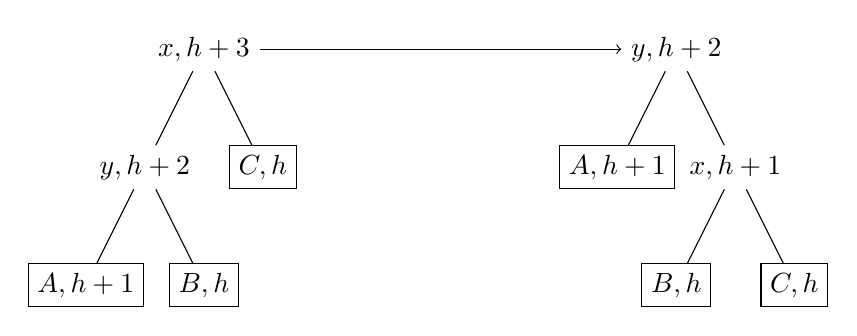
\begin{tikzpicture}
        \node (x1) {$x, h + 3$}
            child {
                node {$y, h + 2$}
                child { node [draw] {$A, h + 1$} }
                child { node [draw] {$B, h$} }
            }
            child {
                node [draw] {$C, h$}
            };
        \node (x2) at (6, 0) {$y, h + 2$}
            child {
                node [draw] {$A, h + 1$}
            }
            child {
                node {$x, h + 1$}
                child { node [draw] {$B, h$} }
                child { node [draw] {$C, h$} }
            };
        \draw[->] (x1) -- (x2);
    \end{tikzpicture}

    \vspace{3em}

    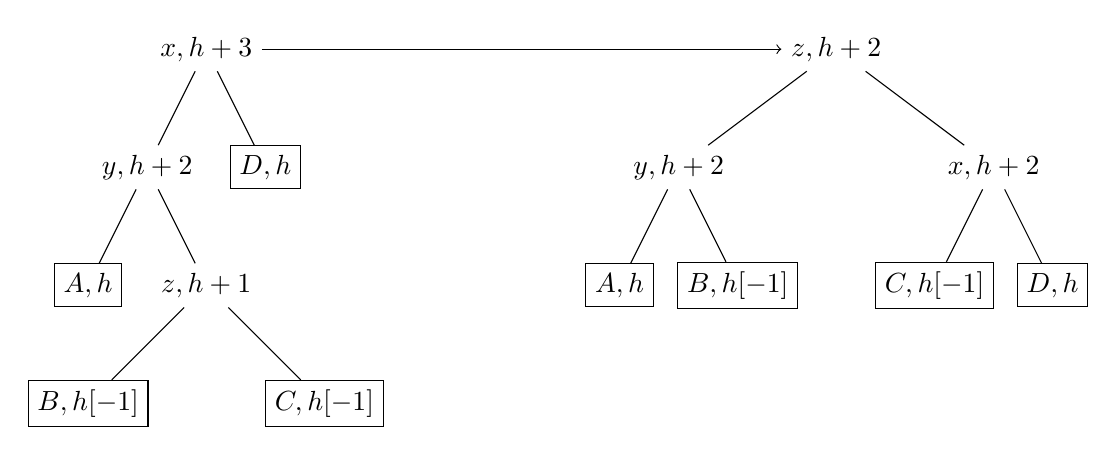
\begin{tikzpicture}
        \node (x1) {$x, h + 3$}
            child {
                node {$y, h + 2$}
                child { node [draw] {$A, h$} }
                child {
                    node {$z, h + 1$}
                    [sibling distance=30mm]
                    child { node [draw] {$B, h [- 1]$} }
                    child { node [draw] {$C, h [- 1]$} }
                }
            }
            child {
                node [draw] {$D, h$}
            };

        \node (x2) at (8, 0) {$z, h + 2$}
            [level 1/.style={sibling distance=40mm}]
            [level 2/.style={sibling distance=15mm}]
            child {
                node {$y, h + 2$}
                child { node [draw] {$A, h$} }
                child { node [draw] {$B, h[-1]$} }
            }
            child {
                node {$x, h + 2$}
                child { node [draw] {$C, h[-1]$} }
                child { node [draw] {$D, h$} }
            };

        \draw[->] (x1) -- (x2);
    \end{tikzpicture}
\end{center}

Докажем, что высота АВЛ-дерева из $n$ вершин --- $\O(\log n)$:
очевидно, при высоте $h$ в дереве не более $2^h - 1$ вершин.
Рассмотрим минимальное количество вершин.
Будем строить АВЛ-дерево, зависящее от высоты, $S(h)$,
следующим образом:

\begin{align*}
    S(0) & = Z \text{ --- null} \\
    S(1) & = \langle Z; Z \rangle \text{ --- лист} \\
    S(h + 2) & = \langle S(h); S(h + 1) \rangle \\
\end{align*}

\begin{statement}
    $S(h)$ --- минимальное АВЛ-дерево высоты $h$.
\end{statement}
\begin{proof}
    Очевидно, $S(0)$ и $S(1)$ минимальны и единственны.

    Пусть доказано, что $S(h)$ и $S(h + 1)$ минимальны.
    АВЛ-дерево высоты $h + 2$ будет иметь два поддерева
    --- высоты $h + 1$ и $h$ или $h + 1$.
    $S(h + 1)$ содержит $S(h)$, поэтому
    $|S(h + 1)| > |S(h)|$, следовательно,
    $S(h)$ --- минимальное возможное поддерево высоты
    $h$ или $h + 1$.

    Тогда
    \begin{align*}
        \forall T \mid h(T) = h + 2 :
        |T| & \geq 1 + \min(|S(h)|; |S(h + 1)|) + |S(h + 1)| = \\
        & = 1 + |S(h)| + |S(h + 1)| = \\
        & = |S(h + 2)| \\
    \end{align*}

    Следовательно, $S(h + 2)$ --- минимальное
    АВЛ-дерево высоты $h + 2$.
\end{proof}

При этом из формулы видно, что
$|S(h + 2)| \geq F(h + 2)$,
и известно, что
\[
    F(n) = \frac{\phi^n - \phi^{-n}}{\sqrt{5}} \in \Theta(\phi^n)
\]

Следовательно,
\begin{gather*}
    \Theta(\phi^n) \leq |S(h)| \leq 2^h - 1 \\
    h(n) \in \Theta(\log n) \\
\end{gather*}
\qed

    \section{Splay-дерево}
Splay-дерево: дерево, которое остаётся сбалансированным
в среднем и при этом не хранит никакой
дополнительной информации в вершинах;
реализация основных операций через операцию splay;
верхняя оценка $\O(\log n)$ на среднюю стоимость операций.

\subsection{Splay}
Операция splay --- перемещение
искомой вершины $x$ в корень,
делится на 3 случая:

\noindent
\begin{minipage}{\textwidth}
    Родитель $x$ --- корень,
    тогда один поворот:

    \begin{center}
        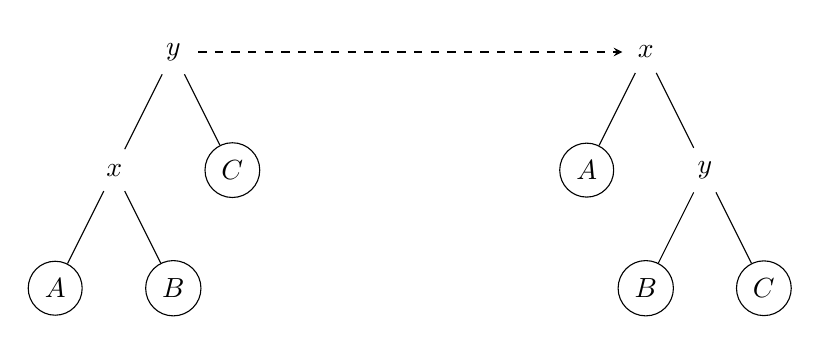
\begin{tikzpicture}[every node/.style={circle}]
            \node (x1) {$y$}
                child {
                    node {$x$}
                    child { node [draw] {$A$} }
                    child { node [draw] {$B$} }
                }
                child { node [draw] {$C$} };

            \node (x2) at (6, 0) {$x$}
                child { node [draw] {$A$} }
                child {
                    node {$y$}
                    child { node [draw] {$B$} }
                    child { node [draw] {$C$} }
                };

            \draw[->,dashed,>=stealth] (x1) -- (x2);
        \end{tikzpicture}
    \end{center}
\end{minipage}

\vspace{3em}

\noindent
\begin{minipage}{\textwidth}
    И $x$, и родитель --- левые (правые) дети,
    тогда два верхних поворота (zig-zig):

    \begin{center}
        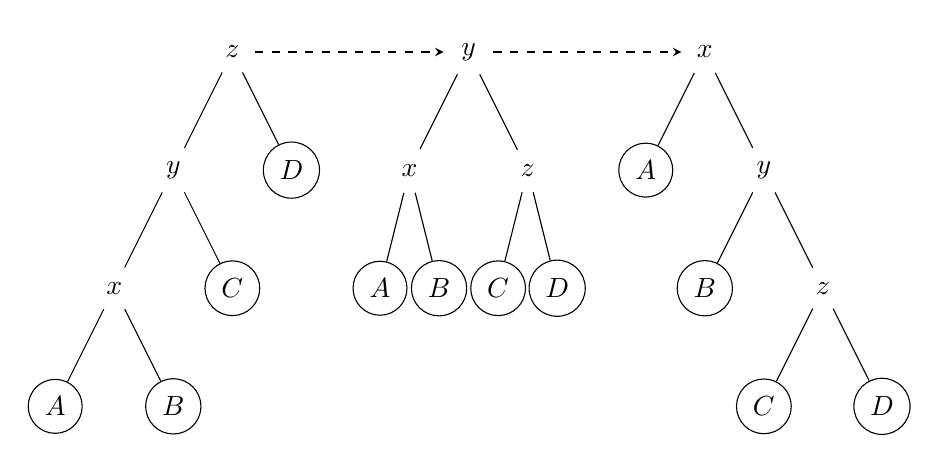
\begin{tikzpicture}[every node/.style={circle}]
            \node (x1) {$z$}
                child {
                    node {$y$}
                    child {
                        node {$x$}
                        child { node [draw] {$A$} }
                        child { node [draw] {$B$} }
                    }
                    child { node [draw] {$C$} }
                }
                child { node [draw] {$D$} };

            \node (x2) at (3, 0) {$y$}
                [level 2/.style={sibling distance=7.5mm}]
                child {
                    node {$x$}
                    child { node [draw] {$A$} }
                    child { node [draw] {$B$} }
                }
                child {
                    node {$z$}
                    child { node [draw] {$C$} }
                    child { node [draw] {$D$} }
                };

            \node (x3) at (6, 0) {$x$}
                child { node [draw] {$A$} }
                child {
                    node {$y$}
                    child { node [draw] {$B$} }
                    child {
                        node {$z$}
                        child { node [draw] {$C$} }
                        child { node [draw] {$D$} }
                    }
                };

            \draw[->,dashed,>=stealth] (x1) -- (x2);
            \draw[->,dashed,>=stealth] (x2) -- (x3);
        \end{tikzpicture}
    \end{center}
\end{minipage}

\vspace{3em}

\noindent
\begin{minipage}{\textwidth}
    $x$ --- правый ребёнок левого ребёнка (или наоборот),
    тогда сначала нижний поворот, потом верхний (zig-zag):

    \begin{center}
        \begin{tikzpicture}
            \node (x1) {$z$}
                child {
                    node {$y$}
                    child { node {$A$} }
                    child {
                        node {$x$}
                        child { node {$B$} }
                        child { node {$C$} }
                    }
                }
                child { node {$D$} };

            \node (x2) at (4, 0) {$z$}
                child {
                    node {$x$}
                    child {
                        node {$y$}
                        child { node {$A$} }
                        child { node {$B$} }
                    }
                    child { node {$C$} }
                }
                child { node {$D$} };

            \node (x3) at (8, 0) {$x$}
                [level 2/.style={sibling distance=7.5mm}]
                child {
                    node {$y$}
                    child { node {$A$} }
                    child { node {$B$} }
                }
                child {
                    node {$z$}
                    child { node {$C$} }
                    child { node {$D$} }
                };

            \draw[->,dashed,>=stealth] (x1) -- (x2);
            \draw[->,dashed,>=stealth] (x2) -- (x3);
        \end{tikzpicture}
    \end{center}
\end{minipage}

После каждой операции поиска (find) выполняется splay.

Разделение дерева (split) --- find, splay,
дальше удаляем одно из рёбер из корня и возвращаем
деревья.

Слияние двух деревьев (merge),
если в одном все элементы меньше другого:
splay от самого большого элемента меньшего дерева,
он оказывается в корне, правого ребёнка у него нет,
подвешиваем к нему второе дерево.

Добавление элемента (add):
разделяем дерево по значению элемента,
затем подвешиваем оба поддерева к новой вершине.

\begin{definition}
    Ранг вершины $x$
    --- это $r(x) = \log_2 S(x)$,
    где $C(x)$ --- количество вершин в поддереве с корнем $x$.
\end{definition}

Будем считать сумму рангов вершин как

\begin{theorem}
    Амортизированное время операции splay
    на дереве с корнем $t$ и искомой вершиной $x$
    --- $T \le 3r(t) - 3r(x) + 1$.
\end{theorem}
\begin{proof}
    Пусть $r'(x)$ --- ранг после операции,
    $y$ --- предок $x$, а $z$ --- предок $y$ (если есть).

    \paragraph{zig}
    Меняются ранги двух вершин,
    \begin{gather*}
        T = 1 + r'(x) + r'(y) - r(x) - r(y) \\
        r'(y) < r(y) \Rightarrow T \le 1 + r'(x) - r(x) = \\
        = 1 + r(y) - r(x) = 1 + r(t) - r(x) \le \\
        \le 1 + 3 r(t) - 3 r(x)
    \end{gather*}

    \paragraph{zig-zig}
    Меняются ранги $x$, $y$, $z$.
    \begin{gather*}
        T = 2 + r'(x) + r'(y) + r'(z) - r(x) - r(y) - r(z) = \\
        = 2 + r'(y) + r'(z) - r(x) - r(y) \le \\
        \le 2 + r'(y) + r'(z) - 2 r(x) \le \\
        \le 2 + r'(x) + r'(z) - 2 r(x)
    \end{gather*}

    \begin{gather*}
        (r(x) - r'(x)) + (r'(z) - r'(x)) = \\
        = \log_2 \frac{C(x)}{C'(x)} + \log_2 \frac{C'(z)}{C'(x)} = \\
        = \log_2 \frac{1 + |A| + |B|}{3 + |A| + |B| + |C| + |D|}
        + \log_2 \frac{1 + |C| + |D|}{3 + |A| + |B| + |C| + |D|}
    \end{gather*}

    Сумма выражений под логарифмами не превосходит 1.
    \[
        4ab = (a + b)^2 - (a - b)^2 \le (a + b)^2
    \]
    Поэтому произведение выражений под логарифмами
    не превосходит $1/4$, следовательно,
    \begin{gather*}
        \log_2 \frac{1 + |A| + |B|}{3 + |A| + |B| + |C| + |D|}
        + \log_2 \frac{1 + |C| + |D|}{3 + |A| + |B| + |C| + |D|} = \\
        = \log_2 \parens{
            \frac{1 + |A| + |B|}{3 + |A| + |B| + |C| + |D|} \cdot
            \frac{1 + |C| + |D|}{3 + |A| + |B| + |C| + |D|}} \le \\
        \le \log_2 \frac{1}{4} \le -2
    \end{gather*}

    \begin{gather*}
        T \le 2 + r'(x) + r'(z) - 2r(x) = \\
        = 3 (r'(x) - r(x)) - 3 (r'(x) - r(x)) + 2 + r'(x) + r'(z) - 2r(x) = \\
        = 3 (r'(x) - r(x)) + 2 - 2 r'(x) + r(x) + r'(z) \le \\
        \le 3 (r'(x) - r(x)) + 2 + (-2) = \\
        = 3 (r'(x) - r(x)) \le 1 + 3 r(t) - 3 r(x)
    \end{gather*}

    \paragraph{zig-zag}
    Меняются ранги $x$, $y$, $z$.
    \begin{gather*}
        T = 2 + r'(x) + r'(y) + r'(z) - r(x) - r(y) - r(z) = \\
        = 2 + r'(y) + r'(z) - r(x) - r(y) \le \\
        \le 2 + r'(y) + r'(z) - 2 r(x)
    \end{gather*}

    Аналогично,
    \begin{gather*}
        (r'(y) + r'(z) - 2 r(x)) - 2 (r'(x) - r(x)) = \\
        = r'(y) + r'(z) - 2 r'(x) = \\
        = \log_2 (1 + |A| + |B|) + \log_2 (1 + |C| + |D|)
        - 2 \log_2 (3 + |A| + |B| + |C| + |D|) = \\
        = \log_2 \frac{1 + |A| + |B|}{3 + |A| + |B| + |C| + |D|}
        + \log_2 \frac{1 + |C| + |D|}{3 + |A| + |B| + |C| + |D|} \le \\
        \le \log_2 \frac{1}{4} = -2
    \end{gather*}

    Поэтому
    \begin{gather*}
        T \le 2 + r'(y) + r'(z) - 2 r(x) = \\
        = 2 + r'(y) + r'(z) - 2 (r'(x) - r(x)) + 2 (r'(x) - r(x)) \le \\
        \le 2 + (-2) + 2 r'(x) - 2 r(x) = \\
        = 2 r'(x) - 2 r(x) \le 1 + 3 r'(x) - 3 r(x)
    \end{gather*}

    Таким образом, во всех трёх случаях
    $T \le 1 + 3 r(t) - 3 r(x)$.
\end{proof}

Следовательно, суммарное амортизированное время операции splay
\[ T \le 1 + 3 \log_2 n - 3 \log_2 C(x) \in \O(\log n) \]

    \section{Декартово дерево}
Декартово дерево: построение декартова дерева за линейное время
(при предварительно отсортированных ключах),
реализация операций вставки и удаления через split и merge.
Treap: верхняя оценка $\O(\log n)$ на мат. ожидание
глубины конкретной вершины, глубины средней вершины,
глубины дерева.
Использование неявного ключа, rope.

\subsection{Решение}
Декартово дерево --- двоичное дерево поиска по ключу
и одновременно куча по приоритету.

Декартово дерево существует и единственно
для любого набора различных ключей и приоритетов,
доказательство --- алгоритм построения за квадрат
(взять в наборе максимальный приоритет,
это будет корень дерева,
все ключи меньше него слева,
все ключи больше него справа,
повторить рекурсивно для обоих поддеревьев).

При предварительно отсортированных ключах
можно построить за линейное время:
проходим по вершинам слева направо,
имеем 3 случая
(ось абсцисс --- ключ, ось ординат --- приоритет):

\bigskip

\noindent
\begin{minipage}{\textwidth}
    \begin{center}
        Вершина добавляется к существующей самой правой:

        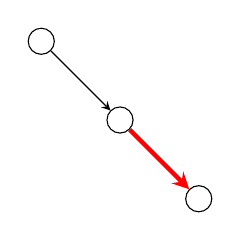
\begin{tikzpicture}[
            every node/.style={draw,circle},
            every path/.style={->,>=stealth}
            ]
            \node (x1) at (1, 3) {};
            \node (x2) at (2, 2) {};
            \node (x3) at (3, 1) {};
            \draw[->] (x1) -- (x2);
            \draw[->,ultra thick,red] (x2) -- (x3);
        \end{tikzpicture}
    \end{center}
\end{minipage}

\bigskip

\noindent
\begin{minipage}{\textwidth}
    \begin{center}
        Вершина становится новым корнем:

        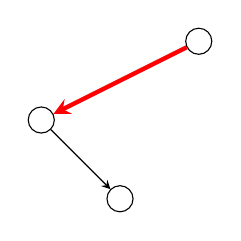
\begin{tikzpicture}[
            every node/.style={draw,circle},
            every path/.style={->,>=stealth}
            ]
            \node (x1) at (1, 2) {};
            \node (x2) at (2, 1) {};
            \node (x3) at (3, 3) {};
            \draw (x1) -- (x2);
            \draw[ultra thick,red] (x3) -- (x1);
        \end{tikzpicture}
    \end{center}
\end{minipage}

\bigskip

\noindent
\begin{minipage}{\textwidth}
    \begin{center}
        Часть дерева переподвешивается к вершине:

        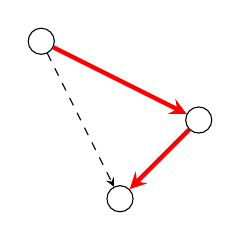
\begin{tikzpicture}[
            every node/.style={draw,circle},
            every path/.style={->,>=stealth}
            ]
            \node (x1) at (1, 3) {};
            \node (x2) at (2, 1) {};
            \node (x3) at (3, 2) {};
            \draw[dashed] (x1) -- (x2);
            \draw[ultra thick,red] (x3) -- (x2);
            \draw[ultra thick,red] (x1) -- (x3);
        \end{tikzpicture}
    \end{center}
\end{minipage}

\bigskip

Можно заметить, что проход наверх по каждому ребру
произойдёт не более одного раза, а количество
всех рёбер --- $n - 1$.
Поэтому мы идём слева направо по ключам,
и время построения декартова дерева --- $\O(n)$.

Операции split и merge:

\noindent
\begin{minipage}{\textwidth}
    \begin{algorithmic}
        \Function{split}{$T, v$}
            \LComment{Всё примерно очевидно}
            \If{$T = \None$}
                \Return $\langle \None; \None \rangle$
            \EndIf
            \State $x$ --- ключ в корне
            \State $p$ --- приоритет в корне
            \State $L$ --- левое поддерево
            \State $R$ --- правое поддерево
            \If{$x < v$}
                \State $\langle T_l; T_r \rangle \gets \Call{split}{R, x}$
                \State $T_n \gets \Call{node}{x, p, L, T_l}$
                \State \Return $\langle T_n; T_r \rangle$
            \Else
                \State $\langle T_l; T_r \rangle \gets \Call{split}{L, x}$
                \State $T_n \gets \Call{node}{x, p, T_r, R}$
                \State \Return $\langle T_l; T_n \rangle$
            \EndIf
        \EndFunction
    \end{algorithmic}
\end{minipage}

\bigskip

\noindent
\begin{minipage}{\textwidth}
    \begin{algorithmic}
        \Function{merge}{$T_1, T_2$}
            \Comment{$\forall x \in T_1.~\forall y \in T_2.~x \leq y$}
            \If{$T_1 = \None$}
                \Return $T_2$
            \EndIf
            \If{$T_2 = \None$}
                \Return $T_1$
            \EndIf
            \State $x_1$ --- значение в корне первого поддерева
            \State $x_2$ --- значение в корне второго поддерева
            \State $p_1$ --- приоритет корня первого поддерева
            \State $p_2$ --- приоритет корня второго поддерева
            \State $L_1$ --- левое поддерево первого поддерева
            \State $L_2$ --- левое поддерево второго поддерева
            \State $R_1$ --- правое поддерево первого поддерева
            \State $R_2$ --- правое поддерево второго поддерева
            \If{$p_1 < p_2$}
                \State $T_n \gets \Call{merge}{T_1, L_2}$
                \State \Return $\Call{node}{x_2, p_2, T_n, R_2}$
            \Else
                \State $T_n \gets \Call{merge}{T_2, R_1}$
                \State \Return $\Call{node}{x_1, p_1, L_1, T_n}$
            \EndIf
        \EndFunction
    \end{algorithmic}
\end{minipage}

Тогда добавление и удаление очевидно реализуются
через split и merge.

\begin{definition}
    Дуча, treap, курево, дерамида --- декартово дерево,
    построенное на независимых случайных приоритетах.
\end{definition}

\begin{theorem}
    Математическое ожидание высоты дерамиды --- $\O(\log n)$.
\end{theorem}
\begin{proof}
    Существует однозначное соответствие между дерамидами
    и деревьями быстрой сортировки.
    Считая оценку для глубины рекурсии быстрой сортировки доказанной,
    получаем оценку для глубины дерамиды.
\end{proof}

Декартово дерево по неявному ключу:
храним количество вершин в левом поддереве,
ключ --- количество вершин, предшествующих данной,
считаем его для вершины по мере спуска к ней.
Очевидно, все свойства выполняются.

    \section{Хеширование}
Прямая адресация.
Коллизии.
Разрешение коллизий методом цепочек,
методом последовательных проб и методом двойного хеширования.
Гипотеза равномерного хеширования.
Оценка времени поиска в хеш-таблице при
использовании метода цепочек для гипотезы
равномерного хеширования.
Примеры хеш-функций.

\subsection{Хеш-таблица}
Прямая адресация --- ключи сами являются целыми числами
из ограниченного диапазона $[0; m - 1]$, и $m$ небольшое.
Множество --- просто массив битов,
словарь --- массив ссылок (или объектов)
и специальных нулевых значений.

Хотим, чтобы размер таблицы был $\O(n)$,
где $n$ --- количество ключей.

Хеш-функция --- из множества ключей в
конечное множество индексов $h: K \to \{0, \ldots, m - 1\}$.
$h(k)$ --- хеш-код ключа $k$.
Поскольку хеш-кодов меньше, чем ключей,
то возникают \emph{коллизии}
--- когда $h(k_1) = h(k_2)$, но $k_1 \ne k_2$.
Коллизии неизбежны, и их обработка --- \emph{разрешение коллизий}.

\bigskip

Метод цепочек: в каждой ячейке (,,бакете``) хеш-таблицы
хранится список ключей с таким хеш-кодом.
Время добавления, удаления, поиска --- $\O(l)$,
где $l$ --- количество ключей в ячейке,
поэтому хотим как можно меньше коллизий.

\bigskip

Открытая адресация (метод последовательных проб):
ключу соответствует не ячейка,
а последовательность ячеек, получаемая как
\[ h(k, 0), h(k, 1), \ldots, h(k, m - 1) \]

При удалении нужно хранить в ячейке флаг, что значение было удалено.
Самый простой вариант новой хеш-функции:
\[ h(k, i) = (h(k) + i) \Mod m \]
Но тут цепочки близких ячеек таблицы ,,склеиваются``.

Более сложный --- \emph{двойное хеширование}:
\[ h(k, i) = (h_1(k) + i \cdot h_2(k)) \Mod m \]
Нужно обеспечить, чтобы для фиксированного ключа элементы
последовательности не повторялись.
Для этого $m$ можно выбрать простым,
тогда подойдёт любая $h_2 : K \to [1; m - 1]$ (не с 0!).

\subsection{Примеры хеш-функций}
Равномерно распределённые вещественные числа на $[0; 1)$:
\[ h(k) = \floor{mk} \]

Целые числа:
\[ h(k) = k \Mod m \]

Более качественное перемешивание целых чисел
--- мультипликативный метод:
\[ h(k) = \floor{m \cdot \{ck\}} \]
где $\{x\} = x - \floor{x}$, $c$ --- некоторая вещественная константа,
в идеале --- иррациональная, например, $\sqrt{2}$ или $\pi$.
Можно обобщить этот метод на пару:
\[ h(k_1, k_2) = \floor{m \cdot \{c_1 k_1 + c_2 k_2\}} \]
при этом $c_1$ и $c_2$ стоит выбирать линейно независимыми
над $\mathds{Q}$, например, $\sqrt{2}$ и $\sqrt{3}$.

Последовательности целых чисел (например, строки)
--- полиномиальный метод:
\[ h(a) = (a_0 + a_1 x + \ldots + a_n x^n) \Mod m \]
где $x$ --- некоторое взаимнопростое с $m$ число.

Кортежи разнотипных значений --- посчитать хеши
отдельных значений, дальше скомбинировать
полиномиальным или мультипликативным методом.

\subsection{Гипотеза равномерного хеширования}
Коэффициент заполнения таблицы $\alpha = n/m$.
Для любой хеш-функции можно подобрать набор ключей
с большим количеством коллизий.

\emph{Гипотеза равномерного хеширования}:
хеш-коды равномерно распределены на
множестве $\{0, \ldots, m - 1\}$,
а хеш-коды разных ключей независимы.

\begin{theorem}
    В предположении гипотезы равномерного хеширования
    среднее время безуспешного поиска в методе цепочек
    --- $\Theta(1 + \alpha)$.
\end{theorem}
\begin{proof}
    Мы должны полностью просмотреть ячейку по хеш-коду $h(k)$.
    Обозначим длину $i$-й цепочки как $l(i)$.
    Тогда математическое ожидание длины цепочки
    \[ l(h(k)) = \frac{1}{m} \sum_{i=0}^{m-1} l(i) = \frac{n}{m} = \alpha \]

    Мы всегда делаем хотя бы одну операцию, отсюда берётся 1.
    Поэтому $\Theta(1 + \alpha)$.
\end{proof}


\begin{theorem}
    В предположении гипотезы равномерного хеширования
    среднее время успешного поиска в методе цепочек
    --- $\Theta(1 + \alpha)$.
\end{theorem}
\begin{proof}
    Пусть были добавлены ключи $k_1, \ldots, k_n$
    в таком порядке.
    Пусть
    \[
        X(i, j) =
        \begin{cases}
            1 & h(k_i) = h(k_j) \\
            0 & h(k_i) \ne h(k_j) \\
        \end{cases}
    \]
    По гипотезе равномерного хеширования
    $\E[X(i, j)] = 1/m$ для $i \ne j$.

    Предположим, что ищем ключ $k_i$.
    Пусть элемент в ячейку добавляется в начало списка
    (т.е. становится головой односвязного).
    Тогда количество элементов,
    которые будут просмотрены,
    равно $X(i, i) + X(i, i + 1) + \ldots + X(i, n)$.

    Тогда среднее время по всем $i$ и по
    распределению $X(i, j)$:

    \begin{gather*}
        \frac{1}{n} \sum_{i=1}^n \E \brackets{\sum_{j=i}^n X(i, j)}
        = \frac{1}{n} \sum_{i=1}^n \parens{1 + \sum_{j = i + 1}^n \E X(i, j)} = \\
        = 1 + \frac{1}{n} \sum_{i=1}^n \sum_{j = i + 1}^n \frac{1}{m}
        = 1 + \frac{1}{n} \sum_{i=1}^n \frac{n - i}{m} = \\
        = 1 + \frac{1}{mn} \parens{n^2 - \frac{n (n + 1)}{2}}
        = 1 + \frac{1}{mn} \parens{n^2 - \frac{n (n + 1)}{2}} = \\
        = 1 + \frac{1}{2mn} \parens{n^2 - n}
        = 1 + \frac{n}{2m} - \frac{1}{2m} \in \Theta(1 + \alpha)
    \end{gather*}
\end{proof}

    \section{Универсальные семейства хеш-функций}
Построение универсального семейства для
целочисленных ключей и для строк.
Оценка времени поиска в хеш-таблице
при использовании метода цепочек для универсального семейства.
Совершенное хеширование с помощью
универсального семейства хеш-функций.

\subsection{Решение}
Множество функций $\cH$
из множества ключей $\mathcal{K}$
в $\{0, \ldots, m - 1\}$
называется
\emph{универсальным семейством хеш-функций},
если для любой пары различных ключей
$k_1$ и $k_2$
\[ \Pr_{h \in \cH} \brackets{h(k_1) = h(k_2)} \le \frac{1}{m} \]
(хеш-функция случайно выбирается один раз)

\begin{theorem}
    Среднее время безуспешного поиска в хеш-таблице при
    универсальном хешировании составляет $\Theta(1 + \alpha)$.
\end{theorem}
\begin{proof}
    \[
        X(i) =
        \begin{cases}
            1 & h(k_i) = h(k) \\
            0 & h(k_i) \ne h(k) \\
        \end{cases}
    \]

    По определению универсального семейства,
    и поскольку $k$ отсутствует в хеш-таблице
    $\E_h(X(i)) \le 1 / m$.

    Поэтому
    \begin{gather*}
        \E \brackets{\sum_{i=1}^n X(i)}
        = \sum_{i=1}^n \E X(i)
        \le \frac{n}{m} = \alpha
    \end{gather*}

    Хотя бы одно действие мы точно произведём,
    поэтому $\Theta(1 + \alpha)$.
\end{proof}

\begin{theorem}
    Среднее время успешного поиска в хеш-таблице при
    универсальном хешировании составляет $\Theta(1 + \alpha)$.
\end{theorem}
\begin{proof}
    Аналогично безуспешному поиску,
    но однин из $X(i)$ будет строго 1,
    поэтому
    \begin{gather*}
        \E \brackets{\sum_{i=1}^n X(i)}
        = \sum_{i=1}^n \E X(i)
        \le 1 + \frac{n - 1}{m} \in \Theta(1 + \alpha)
    \end{gather*}
\end{proof}

\subsection{Пример}
\begin{theorem}
    Путь $K = \{0, \ldots, n\}$.
    Выберем простое $p > n$.
    Тогда семейство $\cH$,
    состоящее из функций
    \[ h_{a, b}(k) = \Bigl( (ak + b) \Mod p \Bigr) \Mod m \]
    для $a = 1, \ldots, p - 1$ и $b = 0, \ldots, p - 1$
    будет универсальным.
\end{theorem}
\begin{proof}
    Рассмотрим $k_1 \ne k_2$.
    \begin{align*}
        & t_1 = (ak_1 + b) \Mod p &
        & t_2 = (ak_2 + b) \Mod p \\
    \end{align*}

    Т.к. $k_1 \ne k_2$, то $t_1 \ne t_2$.
    Если предположить, что $t_1 = t_2$,
    то
    \begin{gather*}
        ak_1 + b \equiv ak_2 + b \pmod{p} \\
        a(k_1 - k_2) \equiv 0 \pmod{p} \\
        a \ne 0 \Rightarrow k_1 = k_2 \\
    \end{gather*}

    По $t_1, t_2, k_1, k_2$ можно однозначно восстановить $a, b$:
    \begin{gather*}
        t_1 - t_2 \equiv a(k_1 - k_2) \pmod{p} \\
        a \equiv (t_1 - t_2) \cdot (k_1 - k_2)^{-1} \pmod{p} \\
        b \equiv t_1 - a k_1 \pmod{p} \\
    \end{gather*}
    (кольцо по модулю $p$ --- поле, в нём есть деление).

    При всех возможных парах $a, b$
    каждая пара $t_1, t_2$ встречается ровно один раз.
    Тогда если выбирать $h_{a, b}$ случайно и равномерно из $\cH$,
    то пары $t_1, t_2$ будут случайно и равномерно
    распределены на $\{0, \ldots, p - 1\}$,
    при этом $t_1 \ne t_2$.

    Тогда вероятность того, что хеш-коды ключей совпадут,
    равна вероятности того, что два различных числа
    из $\{0, \ldots, p - 1\}$ окажутся равны по модулю $m$.
    Для фиксированного $t_1$ количество таких $t_2$ не превосходит
    \[
        \ceil{\frac{p}{m}} - 1
        \le \frac{p + m - 1}{m} - 1
        = \frac{p - 1}{m}
    \]

    Тогда вероятность получить коллизию равна
    \[
        \frac{1}{p} \cdot \frac{p - 1}{m} \le \frac{1}{m}
    \]
\end{proof}

\subsection{Совершенное хеширование}
Хотим для статического поиска иметь
поиск за строгое $\O(1)$
и $\O(n)$ памяти.
Для этого будем использовать таблицы второго уровня
с разными хеш-функциями вместо списков.
Скажем, что $n_i$ --- число ключей,
попавших в $i$-ю первичную ячейку.

\begin{theorem}
    \label{thm:06-1}
    При использовании универсального хеширования
    для хеш-таблицы размера $m = n^2$ вероятность
    возникновения коллизий не более $1/2$.
\end{theorem}
\begin{proof}
    Мат. ожидание количества коллизий
    \[
        \E X \leq \binom{n}{2} \cdot \frac{1}{m}
        = \frac{n(n - 1)}{2} \cdot \frac{1}{n^2} < \frac{1}{2}
    \]

    По неравенству Маркова
    \[
        \Pr \brackets{X \geq 1} \leq \frac{\E X}{1}
        < \frac{1}{2}
    \]
\end{proof}

\begin{theorem}
    \label{thm:06-2}
    При $m = n$
    \[
        \Pr \brackets{\sum_{i=0}^{n-1} n_i^2 \geq 4n} \leq \frac{1}{2}
    \]
\end{theorem}
\begin{proof}
    Покажем, что
    \[
        \E \brackets{\sum_{i=0}^{n-1} n_i^2} < 2n
    \]

    \begin{gather*}
        n_i^2 = n_i + 2 \binom{n_i}{2} \\
        \E \brackets{\sum_{i=0}^{n-1} n_i^2}
        = \E \brackets{\sum_{i=0}^{n-1} n_i + 2 \sum_{i=0}^{n-1} \binom{n_i}{2}}
        = n + 2 \E \brackets{\sum_{i=0}^{n-1} \binom{n_i}{2}} \leq \\
        \brackets{\text{вероятность коллизии не превосходит $1/m = 1/n$}} \\
        \leq n + 2 \binom{n}{2} \cdot \frac{1}{n}
        = n + 2 \cdot \frac{n (n - 1)}{2} \cdot \frac{1}{n}
        = n + n - 1 < 2n
    \end{gather*}

    \[
        \Pr \brackets{\sum_{i=0}^{n-1} n_i^2 \geq 4n}
        \leq \frac{\E \brackets{\sum_{i=0}^{n-1} n_i^2}}{4n}
        < \frac{2n}{4n} = \frac{1}{2}
    \]
\end{proof}

Тогда вероятностный алгоритм
построения совершенной хеш-таблицы:
\begin{enumerate}
    \item Построим хеш-таблицу $H$ и выберем хеш-функцию
    $h : K \to \{0, \ldots, m - 1\}$
    так, чтобы $\sum_{i=0}^{n-1} n_i^2 < 4n$.
    Для этого по теореме~\ref{thm:06-2} в среднем потребуется
    проверить не более двух хеш-функций.

    \item Когда такая $h$ найдена, для каждой $i$-й ячейки $H$
    заводим хеш-таблицу $T_i$ размера $n_i^2$
    и выбираем для неё хеш-функцию $g_i : K \to \{0, \ldots, n^2 - 1\}$
    так, чтобы у неё не было коллизий на множестве ключей,
    для которых $h(k) = i$.
    Для этого по теореме~\ref{thm:06-1} в среднем потребуется
    проверить не более двух хеш-функций.
\end{enumerate}

Полученный алгоритм построения работает за $\O(n)$,
требует $\O(n)$ памяти и даёт поиск за строгие $\O(1)$.

    \section{Числовые алгоритмы}
Cложение, умножение, деление длинных чисел.
Модульная арифметика: сложение, умножение,
возведение в степень, алгоритм Евклида,
расширенный алгоритм Евклида, деление.

\subsection{Алгоритмы арифметики}
Числа представляются как двоичные строки.
$n$ --- длина числа в битах.

Сложение --- очевидный алгоритм за $\O(n)$.

В процессорах умножение обычно
реализуется следующим алгоритмом в столбик
за $\O(n^2)$:
\begin{minted}{rust}
fn mul(mut a: Int, mut b: Int) -> Int {
    let mut r: Int = 0;
    for _ in 0..Int::BITS {
        if b & 1 == 1 {
            r += a;
        }
        a <<= 1;
        b >>= 1;
    }
    r
}
\end{minted}

Деление и получение остатка реализуется
алгоритмом в столбик
за $\O(n^2)$
(точнее, за $\O(n \cdot (n - m))$,
где $m$ --- старший бит $b$, считая с 0, $m < n$):
\begin{minted}{rust}
fn div_rem(mut a: Int, mut b: Int) -> (Int, Int) {
    let mut r: Int = 0;
    let mut maxbit = 0;
    for i in 0..Int::BITS {
        if b & (1 << i) != 0 {
            maxbit = i;
        }
    }
    for i in (0..Int::BITS - maxbit).rev() {
        let b = b << i;
        if a >= b {
            r |= 1 << i;
            a -= b;
        }
    }
    (r, a)
}
\end{minted}

Есть алгоритм Карацубы для умножения
за $\O(n^{\log_2 3})$.
Он основан на следующем:
\begin{gather*}
    (ax + b) \cdot (cx + d)
    = ac x^2 + (ad + bc) \cdot x + bd \\
    (a + b) \cdot (c + d)
    = ac + ad + bc + bd \\
    ad + bc = (a + b) \cdot (c + d) - ac - bd
\end{gather*}

Поэтому при дроблении задачи в 2 раза
достаточно провести 3 умножения частей
и $\O(1)$ сложений, а не 4 умножения,
т.е.
\begin{gather*}
    T(n) = 3 \cdot T(n/2) + \O(n) \\
    T(n) \in \O(n^{\log_2 3})
\end{gather*}

Существует алгоритм умножения,
основанный на быстром преобразовании Фурье,
за $\O(n \log n)$.

Базовый алгоритм Евклида:
\begin{minted}{rust}
fn gcd(a: Int, b: Int) -> Int {
    if a < b {
        gcd(b, a)
    } else if b == 0 {
        a
    } else {
        gcd(b, a - b)
    }
}
\end{minted}

Обычно пишут как
\begin{minted}{rust}
fn gcd(a: Int, b: Int) -> Int {
    if b == 0 {
        a
    } else {
        gcd(b, a % b)
    }
}
\end{minted}

\begin{theorem}
    Алгоритм Евклида находит НОД.
\end{theorem}
\begin{proof}
    Пусть $a = bq + r$.
    Пусть $a \equiv 0 \pmod c$
    и $b \equiv 0 \pmod c$.
    Тогда $r \equiv 0 \pmod c$,
    т.к. $r = a - bq$.
    Тогда множества общих делителей
    у $(a, b)$ и у $(b, r)$ совпадают.
\end{proof}

\begin{theorem}[Теорема Безу]
    Всегда существуют целые $x$ и $y$
    такие, что $ax + by = \gcd(a, b)$.
\end{theorem}
\begin{proof}
    Расширенный алгоритм Евклида.
    \begin{minted}{rust}
    fn gcd_ext(a: Int, b: Int) -> (Int, Int, Int) {
        if a < b {
            let (g, x, y) = gcd_ext(b, a);
            (g, y, x)
        } else if b == 0 {
            (a, 1, 0)
        } else {
            let (g, x, y) = gcd_ext(b, a - b);
            (g, y, x - y)
        }
    }
    \end{minted}
\end{proof}

Расширенный алгоритм Евклида можно записать через модуль:
\begin{minted}{rust}
fn gcd_ext_mod(a: Int, b: Int) -> (Int, Int, Int) {
    if b == 0 {
        (a, 1, 0)
    } else {
        let q = a / b;
        let (g, x, y) = gcd_ext_mod(b, a % b);
        (g, y, x - q * y)
    }
}
\end{minted}

\begin{theorem}
    $|x| \le b$ и $|y| \le a$
\end{theorem}
\begin{proof}
    Если $a \equiv 0 \pmod b$,
    то рекурсивный вызов вернёт $(b, 1, 0)$.

    По индукции предположим, что для рекурсивного вызова выполняется.
    Тогда
    \begin{gather*}
        q = \floor{\frac{a}{b}} \\
        r = a \Mod b \\
        \gcd(a, b) = x' \cdot b + y' \cdot r \\
        |x'| \le r \\
        |y'| \le b \\
        x = y' \\
        y = x' - qy' \\
        |x| = |y'| \le b \\
        |y| \le |x'| + |qy'| \le r + qb = a
    \end{gather*}
\end{proof}

Возведение в степень --- алгоритм за $\O(M \log p)$,
где $M$ --- сложность умножения, а $p$ --- степень.

\subsection{Модульная арифметика}
Сложение, умножение, степень --- очевидно.

Деление --- через расширенный алгоритм Евклида
и поиск обратного:
\begin{gather*}
    a / b = a \cdot b^{-1} \\
    b \cdot b^{-1} \equiv 1 \pmod m \\
\end{gather*}

Для существования такого $q$ нужно,
чтобы $\gcd(b, m) = 1$, т.к. иначе
$1 \ne \gcd(b, m) \mid bq$.

Воспользуемся расширенным алгоритмом Евклида и найдём $x$ и $y$:
\[ bx + my \equiv bx \equiv 1 \pmod m \]
это $x$ и будет искомым $q$.
Нужно модифицировать $\gcd$ для использования модульного
сложения и умножения:
\begin{minted}{rust}
fn gcd_ext_mod(a: Int, b: Int, m: Int) -> (Int, Int, Int) {
    if a < b {
        let (g, x, y) = gcd_ext_mod(b, a, m);
        (g, y, x)
    } else if b == 0 {
        (a, 1, 0)
    } else {
        let (g, x, y) = gcd_ext_mod(b, (a + m - b) % m, m);
        (g, y, (x + m - y) % m)
    }
}
\end{minted}

Если $m$ --- простое, то обратный элемент есть всегда.

    \section{Простые числа}
Проверка чисел на простоту.
Числа Кармайкла, малая теорема Ферма.
Генерация случайных простых чисел.
Криптография: схемы с закрытым ключом, RSA.
Необходимые факты теории чисел.

\subsection{Тесты}
\begin{theorem}[Малая теорема Ферма]
    Если $p$ --- простое, и $1 \leq a < p$, то
    \[ a^{p - 1} \equiv 1 \pmod p \]
\end{theorem}
\begin{proof}
    Рассмотрим множество ненулевых остатков от деления на $p$:
    $\{1, \ldots, p - 1\}$.
    При умножении любого из них на $a$ мы получим
    остаток из этого же множества.
    При этом никакие два умножения не дадут один результат,
    т.к. если
    $an \equiv am \pmod p$,
    то $a(n - m) \equiv 0 \pmod p$,
    следовательно, $n = m$.

    Тогда
    \[
        \{1, \ldots, p - 1\}
        = \{ a \cdot 1 \Mod p, \ldots, a \cdot (p - 1) \Mod p \}
    \]

    Перемножим все элементы этого множества:
    \begin{gather*}
        (p - 1)! \equiv a^{p - 1} \cdot (p - 1)! \pmod p \\
        \gcd((p - 1)!, p) = 1 \\
        (p - 1)! \cdot (a^{p - 1} - 1) \equiv 0 \pmod p \\
        a^{p - 1} \equiv 1 \pmod p
    \end{gather*}
\end{proof}

Быстрая проверка на простоту --- тест Ферма:
проверить, подходит ли число под малую лемму Ферма.

\begin{theorem}
    Если $\exists a \mid a^{m - 1} \not \equiv 1 \pmod m \land \gcd(a, m) = 1$,
    то чисел, не проходящих тест, хотя бы половина.
\end{theorem}
\begin{proof}
    Возьмём любое $b \mid b^{m - 1} \equiv 1 \pmod m$.
    Рассмотрим $ab$:
    \[
        (ab)^{m - 1}
        \equiv a^{m - 1} \cdot b^{m - 1}
        \equiv a^{m - 1} \not \equiv 1 \pmod m
    \]

    При этом если $c \ne b, c^{m - 1} \equiv 1 \pmod m$,
    то $ab \ne ac$, т.к. $a$ обратимо.
\end{proof}

Поэтому для случайно взятого $1 < a < m$
шанс ошибки в тесте Ферма не превышает $1/2$,
если число вообще может быть отсеяно этим тестом.

\begin{definition}
    Числа Кармайкла --- составные числа,
    которые всегда проходят тест Ферма.
\end{definition}
Чисел Кармайкла мало: $561 = 3 \cdot 11 \cdot 17$
проходит тест Ферма для всех $a$, взаимно простых с собой.

Тест Рабина-Миллера:
пусть $N$ --- нечётное.
Представим $N - 1 = 2^t \cdot u$,
где $u$ --- нечётное.
Выберем случайное $a$,
вычислим $a^{N - 1} \Mod N$.
Найдём первую единицу в последовательности
\[
    a^u \Mod N,
    a^{2u} \Mod N,
    a^{4u} \Mod N, \ldots,
    a^{N - 1} \Mod N
\]
(а если прошли тест Ферма, то она есть),
посмотрим на предыдущее число.
Если оно не является минус единицей,
то это нетривиальный корень из 1,
и, следовательно, $N$ составное.

Тест Рабина-Миллера с вероятностью $3/4$ обнаруживает
любое составное число, в т.ч. числа Кармайкла.

\subsection{Генерация простых чисел}
Число из $n$ битов имеет вероятность
$\approx 1/(\ln 2^n) \approx 1.44/n$
быть простым.

\begin{theorem}[Закон распределения простых чисел]
    Пусть $\pi(x)$ --- количество простых чисел,
    не превосходящих $x$.
    Тогда
    \[ \lim_{x \to \infty} \frac{\pi(x) \cdot \ln x}{x} = 1 \]
\end{theorem}

Поэтому для генерации простых чисел достаточно
генерировать $n$ бит и проверять на простоту.
На практике теста Ферма для
$a = 2$ достаточно,
но можно и добавить $a = 3, 5, 7, \ldots$.
Среднее количество попыток будет $n$.

Доказательство --- численный эксперимент.
Из первых $25 \cdot 10^9$ чисел
будет $\approx 10^9$ простых
и $\approx 2 \cdot 10^4$ составных,
т.е. шанс ошибки --- $0.002\%$.

\subsection{RSA}
Алиса хочет послать Бобу сообщение,
Боб посылает Алисе открытый ключ,
которым Алиса сможет зашифровать сообщение,
чтобы только Боб мог его расшифровать.
Алгоритм RSA основывается на предположении,
что факторизация числа --- сложная задача.

\begin{theorem}
    Если $p$ и $q$ простые, а $e$ взаимно просто
    с $(p - 1) (q - 1)$, то:
    \begin{enumerate}
        \item Отображение $x \to x^e \mod pq$
        --- перестановка остатков по модулю $pq$
        \item Обратной перестановкой будет $x \to x^d \mod pq$,
        где $e \cdot d \equiv 1 \pmod{pq}$.
        То есть $(x^e)^d \equiv x \pmod{pq}$.
    \end{enumerate}
\end{theorem}
\begin{proof}
    Достаточно доказать второе утверждение,
    т.к. если есть обратное отображение, то само отображение --- перестановка.
    Очевидно, $d$ существует, поскольку $\gcd(e, pq) = 1$.
    Возьмём $d = e^{-1} \pmod{pq}$.
    $ed = 1 + k(p - 1)(q - 1)$.

    По малой теореме Ферма
    $x^{p - 1} \equiv 1 \pmod p$ при $x \ne 0$, поэтому
    \[ x^{1 + k(p - 1)(q - 1)} \equiv x \pmod p \]
    Аналогично $x^{ed} \equiv x \pmod q$.

    Поскольку $\gcd(p, q) = 1$,
    то $x^{ed} \equiv x \pmod{pq}$.
\end{proof}

Тогда можно опубликовать пару $\langle pq; e \rangle$
как \emph{открытый ключ}, и держать $\langle pq; d \rangle$
как \emph{закрытый ключ}.
Тогда
\begin{gather*}
    E(x) = x^e \Mod pq \\
    D(y) = y^d \Mod pq \\
    D(E(x)) = (x^e \Mod pq)^d \Mod pq = (x^e)^d \Mod pq = x
\end{gather*}

Часто берут $e = 3$.

    \section{Быстрое преобразование Фурье}
Быстрое вычисление значений многочлена в точках:
два способа задания многочленов
--- коэффициентами и значениями в точках;
вычисление значений многочлена в точках методом
<<разделяй и властвуй>>;
дискретное преобразование Фурье;
быстрое преобразование Фурье.
Интерполяция: интерполяция в терминах матриц;
матрица Вандермонда;
интерполяция как домножение на обратную матрицу.
Необходимые факты линейной алгебры.

\subsection{Конспект}
Многочлен степени $d$ однозначно задаётся $d + 1$ точкой,
доказательство --- метод интерполяции.
Произведение двух многочленов степени $d$ ---
многочлен степени $2d$.

Заметим, что если мы выбираем точки вида
$x_{2k} = -x_{2k - 1}$,
то можно разделить многочлен
$P(x) = a_0 + a_1 x + a_2 x^2 + \ldots$
в виде $P(x) = P_0(x) + x \cdot P_1(x)$,
где $P_0(x) = a_0 + a_2 x^2 + \ldots$,
а $P_1(x) = a_1 + a_3 x^2 + \ldots$.
Тогда можно посчитать $P(x)$ и $P(-x)$ вместе:
\begin{align*}
    P(x) & = P_0(x) + x \cdot P_1(x) \\
    P(-x) & = P_0(-x) - x \cdot P_1(-x) = \\
    & = P_0(x) - x \cdot P_1(x) \\
\end{align*}

Именно так работает быстрое преобразование Фурье,
только $x$ берутся нетривиальными корнями из 1.
Обычно --- в комплексных числах:
\begin{center}
    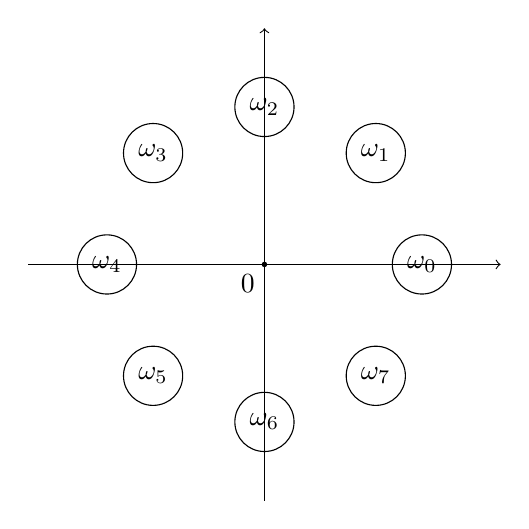
\begin{tikzpicture}
        \foreach \w in {0,...,7} {
            \node[draw,circle] (w\w) at (45*\w : 2cm) {$\omega_{\w}$};
        }
        \draw[->] (-3,0) -- (3,0);
        \draw[->] (0,-3) -- (0,3);
        \fill (0,0) circle (1pt);
        \node[anchor=north east] at (0,0) {$0$};
    \end{tikzpicture}
\end{center}

То есть для $j = 2k \Mod n$
выполняется $\omega_j = \omega_k^2$
и $n = 2^q$.
Иными словами,
$\omega_i = \exp \parens{\frac{2 \pi i}{n}}$.

FFT позволит быстро посчитать точки:

\noindent
\begin{minipage}{\textwidth}
    \begin{algorithmic}
        \State $\omega_N(i) = \exp \parens{\frac{2 \pi i}{N}}$
        \Function{fft}{$n=N, k=0, \Delta=1$}
            \Comment{$k$ --- индекс, $\Delta$ --- шаг индекса}
            \If{$n = 1$}
                \Return $P[k]$
            \EndIf
            \State $P_0(\omega^{2j}) = \Call{fft}{n / 2, k, 2 \Delta}$
            \State $P_1(\omega^{2j}) = \Call{fft}{n / 2, (k + \Delta) \Mod N, 2 \Delta}$
            \For{$j = 0, \ldots, n - 1$}
                \State $P(\omega^j) = P_0(\omega^{2j}) + \omega^j \cdot A_1(\omega^{2j})$
            \EndFor
            \Return $P(\omega^j)$
        \EndFunction
    \end{algorithmic}
\end{minipage}

Очевидно, \textsc{fft} работает за $\O(N \log N)$.

Матричный вид, т.н. матрица Вандермонда:

\[
    \begin{bmatrix}
        P(x_0) \\
        P(x_1) \\
        \ldots \\
        P(x_{n - 1}) \\
    \end{bmatrix}
    =
    \begin{bmatrix}
        1 & x_0 & x_0^2 & \ldots & x_0^{n - 1} \\
        1 & x_1 & x_1^2 & \ldots & x_1^{n - 1} \\
        & & \vdots & & \\
        1 & x_{n - 1} & x_{n - 1}^2 & \ldots & x_{n - 1}^{n - 1} \\
    \end{bmatrix}
    \cdot
    \begin{bmatrix}
        a_0 \\
        a_1 \\
        \ldots \\
        a_{n - 1} \\
    \end{bmatrix}
\]

Интерполяцию можно реализовать домножением на обратную матрицу:
\[
    \frac{1}{n}
    \cdot
    \begin{bmatrix}
        1 & 1 & \ldots & 1 \\
        \omega_0^{-1} & \omega_1^{-1} & \ldots & \omega_{n - 1}^{-1} \\
        \omega_0^{-2} & \omega_1^{-2} & \ldots & \omega_{n - 1}^{-2} \\
        & & \vdots & & \\
        \omega_0^{1 - n} & \omega_1^{1 - n} & \ldots & \omega_{n - 1}^{1 - n} \\
    \end{bmatrix}
    \cdot
    \begin{bmatrix}
        1 & \omega_0 & \omega_0^2 & \ldots & \omega_0^{n - 1} \\
        1 & \omega_1 & \omega_1^2 & \ldots & \omega_1^{n - 1} \\
        & & \vdots & & \\
        1 & \omega_{n - 1} & \omega_{n - 1}^2 & \ldots & \omega_{n - 1}^{n - 1} \\
    \end{bmatrix}
    = ?
\]

Рассмотрим отдельную ячейку $i, j (i \ne j)$:
\[
    \frac{1}{n}
    \sum_{k=0}^{n - 1}
    \omega_k^{-i}
    \cdot
    \omega_k^j
    =
    \frac{1}{n}
    \sum_{k=0}^{n - 1}
    \omega_1^{k(j - i)}
    =
    \frac{1}{n}
    \cdot
    \frac{1 - \omega_1^{n(j - i)}}{1 - \omega_1^{j - i}}
    =
    0
\]

\[
    \frac{1}{n}
    \sum_{k=0}^{n - 1}
    \omega_k^{-j}
    \cdot
    \omega_k^j
    =
    1
\]

Т.е. на главной диагонали единицы,
в остальных ячейках нули.
Получили обратную матрицу.

    \section{Задача линейного программирования и симплекс-метод}
Линейное программирование.
Общий вид задачи, матричная форма и
сведение между различными представлениями.
Вершины: равносильность двух определений и достижение максимума.
Симплекс-метод, нахождение начальной точки.
Двойственность: построение двойственной
задачи, теорема о двойственности --- слабая (с доказательством)
и сильная (без доказательства) формулировки.

\subsection{Задача}
Есть набор переменных, нужно присвоить им вещественные значения
с учётом линейных ограничений
и максимизируя / минимизируя линейную функцию.

\begin{align*}
    &
    \begin{system}
        & \sum_{i=1}^n c_i x_i \to \max \\
        & \forall j \in \{1, \ldots, m\}.~\sum_{i=1}^n a_{ji} x_i \le b_j \\
        & \forall i \in \{1, \ldots, n\}.~x_i \ge 0 \\
    \end{system}
    &&
    \begin{system}
        C^T \cdot X & \to \max \\
        A \cdot X & \le B \\
        X & \ge 0 \\
    \end{system}
\end{align*}

Пример --- максимизация прибыли,
если на складе есть материалы,
из которых производятся товары
заранее известной стоимости.

Стоит обратить внимание, что неравенства нестрогие.

\subsection{Разные виды}
\begin{itemize}
    \item Целевая функция максимизируется или минимизируется
    (эквивалентно, т.к. просто $c_i$ разного знака);

    \item Ограничения неравенством или равенством:
    для $\sum_{i=1}^n a_i x_i \le b$
    вводим $s$ и пишем
    \begin{eqnsystem}
        & \sum_{i=1}^n a_i x_i + s = b \\
        & s \ge 0 \\
    \end{eqnsystem}

    Обратно --- для $A = B$ пишем $A \le B$ и $A \ge B$ ($-A \le -B$);

    \item Неограниченная переменная сводится к двум неотрицательным:
    $x = x^+ - x^-$, $x^+ \ge 0$, $x^- \ge 0$.
\end{itemize}

\paragraph{Стандартный вид:}
целевая функция минимизируется,
все переменные неотрицательные,
ограничения --- уравнения.

\subsection{Двойственная задача}
\paragraph{Пример}
\begin{eqnsystem}
    x_1 + 6 x_2 & \to \max \\
    x_1 & \le 200 \\
    x_2 & \le 300 \\
    x_1 + x_2 & \le 400 \\
    x_1, x_2 & \ge 0 \\
\end{eqnsystem}

Решение этой задачи:
$x_1 = 100, x_2 = 300$,
тогда $x_1 + 6 x_2 = 1900$.
Можно доказать, что это решение, сложив
второе и третье ограничения с коэффициентами 5 и 1:
\begin{gather*}
    5 x_2 + x_1 + x_2 \le 5 \cdot 300 + 400 \\
    x_1 + 6 x_2 \le 1900
\end{gather*}

Хотим найти такие коэффициенты для оценки в общем случае.
Обозначим коэффициенты при неравенствах
как $y_1, y_2, y_3$.
Хотим минимизировать
$y_1 \cdot x_1 + y_2 \cdot x_2 + y_3 \cdot (x_1 + x_2)$,
при этом $y_1, y_2, y_3 \ge 0$
(иначе поменяется знак неравенства).
Тогда получаем неравенство
\[
    (y_1 + y_3) x_1 + (y_2 + y_3) x_2 \le 200 y_1 + 300 y_2 + 400 y_3
\]
При этом хотим, чтобы левая часть совпала с целевой функцией,
т.е.
\[
    x_1 + 6 x_2 \le 200 y_1 + 300 y_2 + 400 y_3
\]
Для этого требуются ограничения
\begin{eqnsystem}
    y_1, y_2, y_3 & \ge 0 \\
    y_1 + y_3 & \ge 1~\text{(неравенство, т.к. $y$ только справа)} \\
    y_2 + y_3 & \ge 6
\end{eqnsystem}

Чтобы оценка была как можно более точной,
нужно минимизировать $200 y_1 + 300 y_2 + 400 y_3$.
Снова получили задачу линейного программирования:
\begin{eqnsystem}
    200 y_1 + 300 y_2 + 400 y_3 & \to \min \\
    y_1 + y_3 & \ge 1 \\
    y_2 + y_3 & \ge 6 \\
    y_1, y_2, y_3 & \ge 0 \\
\end{eqnsystem}

\paragraph{Общий случай}
Всякое решение двойственной задачи
--- оценка для прямой задачи,
поэтому пара решений с совпадающими
значениями будет оптимальной.

Если прямая задача:
\begin{eqnsystem}
    & \sum_{i=1}^n c_i x_i \to \max \\
    & \forall j \in \{1, \ldots, m\}.~\sum_{i=1}^n a_{ji} x_i \le b_j \\
    & \forall i \in \{1, \ldots, n\}.~x_i \ge 0 \\
\end{eqnsystem}

То двойственная --- это оценка для прямой, и будет иметь вид:
\begin{eqnsystem}
    & \sum_{j=1}^m b_i y_i \to \min \\
    & \forall i \in \{1, \ldots, n\}.~\sum_{j=1}^m a_{ji} y_j \ge c_i \\
    & \forall j \in \{1, \ldots, m\}.~y_j \ge 0 \\
\end{eqnsystem}

Матричный вид:
\begin{align*}
    &
    \begin{system}
        C^T \cdot X & \to \max \\
        A \cdot X & \le B \\
        X & \ge 0 \\
    \end{system}
    &&
    \begin{system}
        B^T \cdot Y & \to \min \\
        A^T \cdot Y & \ge C \\
        Y & \ge 0
    \end{system}
\end{align*}

Из матричного вида очевидно,
что двойственная задача к двойственной задаче
--- прямая задача.

\begin{theorem}[Теорема о двойственности]
    Если линейная программа имеет ограниченный
    оптимум, то двойственная программа также
    имеет ограниченный оптимум,
    и они равны.
\end{theorem}

\begin{theorem}[Слабая теорема о двойственности]
    Разница между прямым и двойственным оптимумом
    неотрицательна.
\end{theorem}
\begin{proof}
    \[
        C^T X = X^T C \le X^T A^T Y \le B^T Y
    \]
\end{proof}

\subsection{Симплекс-метод}
Линейные ограничения задают гиперплоскости,
которые содержат грани полиэдра (многогранника),
в котором лежат все точки, попадающие под ограничения.
Ограничения могут быть не замкнуты,
тогда функция может быть бесконечной,
либо точек, попадающих под ограничения,
может не быть.
Если же ограничения замкнуты,
тогда ответ лежит в одной из вершин.

Симплекс-метод:
найти некоторую вершину,
дальше идти в сторону тех соседей,
для которых целевая функция увеличивается.

\begin{definition}
    Вершина в $n$-мерном пространстве
    --- единственная точка пересечения $n$ гиперплоскостей
    (или единственное решение системы из $n$ линейных уравнений).
\end{definition}
\begin{definition}
    Две вершины в $n$-мерном пространстве называются \emph{соседними},
    если у них $(n - 1)$ одинаковое уравнение.
\end{definition}

Если находимся в начале координат,
то у всех соседних вершин все координаты,
кроме одной, нулевые.

Если не находимся в начале координат,
то можно совершить афинное преобразование пространства,
чтобы нормали к плоскостям,
на пересечении которых мы находимся,
задавали новое пространство.
Была целевая функция
$\alpha + C^T X$, стала $c_u + \tilde{C}^T Y$,
где $c_u$ --- значение в вершине $u$.

Тогда глобальный оптимум получается,
когда все преобразованные $\tilde{c}_i \le 0$.

\subsubsection{Как найти начальную вершину}
Ноль не всегда попадает под ограничения.
Пусть есть задача в стандартном виде:
\begin{align*}
    & c^T x \to \min
    && Ax = b
    && x \ge 0
\end{align*}
Считаем, что $b \ge 0$.
Запишем новую линейную программу:
на каждое уравнение введём $z \ge 0$:
$z + Ax = z + b$.
Минимизировать будем
$z_1 + z_2 + \ldots + z_m$.

У такой задачи легко получить
вершину: $z = b, x = 0$.

Если в оптимуме сумма $z$ оказалась нулём,
то все $z_j$ --- нули, следовательно,
найденные $x_i$ подходят под ограничения исходной задачи.

Если же наименьшая сумма больше нуля,
то исходная задача несовместна.

\subsubsection{Неограниченная задача}
На каком-то шаге возникнет
бесконечно удалённая соседняя вершина.
Тогда она будет доказательством,
что оптимум бесконечен.

\subsubsection{Время работы}
$\O(mn)$ за итерацию,
где $m$ --- количество ограничений,
а $n$ --- количество переменных,
потому что на каждом шаге у нас
преобразуется система координат.

Но количество итераций
--- до количества вершин,
т.е. $\binom{m + n}{n}$.
Т.е. симплекс-метод экспоненциален.

    \section{Целочисленное линейное программирование}
ILP: пример для максимального паросочетания
и вершинного покрытия в двудольном графе.
Тотальная унимодулярность:
определение и почему это гарантирует целочисленность решения.
Доказательство теоремы Кёнига через двойственность.

\subsection{Двудольный граф}
Максимальное паросочетание:
каждому ребру $e_j$ назначим $x_j$
--- берём или нет это ребро,
и задача выглядит так:
\begin{eqnsystem}
    & \sum_{j=1}^{|E|} x_j \to \max \\
    & \forall i \le |V|.~\sum_{j=1}^{|E|} a_{ij} x_j \le 1 \\
    % & \forall j \le |E|.~x_j \le 1 \\
    & \forall j \le |E|.~x_j \ge 0 \\
\end{eqnsystem}
где $a_{ij}$ --- инцидентность вершины $v_i$ ребру $e_j$.

Минимальное вершинное покрытие:
каждой вершине $v_i$ назначим $y_i$
--- берём или нет эту вершину.
Задача выглядит так:
\begin{eqnsystem}
    & \sum_{i=1}^{|V|} y_i \to \min \\
    & \forall j \le |E|.~\sum_{i=1}^{|V|} a_{ij} y_i \ge 1 \\
    % & \forall i \le |V|.~y_i \le 1 \\
    & \forall i \le |V|.~y_i \ge 0 \\
\end{eqnsystem}
где $a_{ij}$ --- инцидентность вершины $v_i$ ребру $e_j$.

\begin{theorem}[теорема Кёнига]
    Максимальное паросочетание не больше минимального вершинного покрытия
\end{theorem}
\begin{proof}
    См. задачи линейного программирования выше,
    можно заметить, что если
    $A$ --- матрица инцидентности
    (т.е. $a_{ij}$ --- инцидентность $v_i$ и $e_j$),
    то задачи выглядят как
    \begin{align*}
        &
        \begin{system}
            & 1_{|E|}^T \cdot X \to \max \\
            & A \cdot X \le 1_{|V|} \\
            & X \ge 0 \\
        \end{system}
        &&
        \begin{system}
            & 1_{|V|}^T \cdot Y \to \min \\
            & A^T \cdot Y \ge 1_{|E|} \\
            & Y \ge 0 \\
        \end{system}
    \end{align*}
    Т.е. задачи двойственны друг другу,
    следовательно,
    оптимум минимального вершинного покрытия
    равен оптимуму максимального паросочетания.
\end{proof}

\subsection{Унимодулярность}
Тотальная унимодулярность:
определитель каждой квадратной подматрицы
(в т.ч. с пробелами) --- $\pm 1$ или $0$.
\begin{theorem}
    Все вершины многогранника с тотально унимодулярной
    матрицей целочисленны.
\end{theorem}
\begin{proof}
    Рассмотрим вершину $(x_1, \ldots, x_n)$.
    Её система уравнений:
    \begin{eqnsystem}
    \end{eqnsystem}
\end{proof}

    \section{Задача о максимальном потоке}
Задача о максимальном потоке.
Теорема о минимальном разрезе и максимальном потоке.
Алгоритм Форда-Фалкерсона.
Алгоритм Эдмондса-Карпа (без доказательства корректности).
Двудольное паросочетание через потоки.

    \section{Поиск подстроки в строке}
Наивный алгоритм.
Алгоритм Рабина-Карпа.
$z$-функция, префикс-функция,
алгоритм Кнута-Морриса-Пратта.

\subsection{Конспект}
Наивный алгоритм --- очевидно.

Алгоритм Рабина-Карпа: полиномиальное хеширование.
$\O(n + m)$.

$z$-функция:
$z_i$ --- максимальная длина префикса строки,
который совпадает с префиксом её $i$-го суффикса.
префикс- или $\pi$-функция:
$\pi_i$ --- максимальная длина префикса $(i - 1)$-го префикса строки,
который совпадает с суффиксом её $i$-го префикса.
$z$- и префикс-функцию можно посчитать за $\O(n)$:

\bigskip
\noindent
\begin{minipage}{\textwidth}
\begin{minted}{rust}
pub fn calc_zfun_inplace(s: &[impl Eq], z: &mut [usize]) {
    let n = s.len();
    assert_eq!(n, z.len());
    if n == 0 {
        return;
    }
    z[0] = n;
    if n == 1 {
        return;
    }
    // Поддерживаем самый правый совпадающий с префиксом диапазон,
    // может быть нулевой длины
    let mut l = 1;
    let mut r = 1;
    z[1] = r - l;
    for i in 1..n {
        let mut k = 0;
        if i < r {
            // s[i..r] = s[i - l..r - l]
            k = z[i - l].min(r - i);
        }
        while i + k < n && s[k] == s[i + k] {
            k += 1;
        }
        z[i] = k;
        if i + k > r {
            l = i;
            r = i + k;
        }
    }
}
\end{minted}
\end{minipage}

Пояснение:
\begin{center}
    \begin{tikzpicture}

    \end{tikzpicture}
\end{center}

\bigskip
\noindent
\begin{minipage}{\textwidth}
\begin{minted}{rust}
pub fn calc_pfun_inplace(s: &[impl Eq], p: &mut [usize]) {
    let n = s.len();
    assert_eq!(n, p.len());
    if n == 0 {
        return;
    }
    p[0] = 0;
    for i in 1..n {
        let mut k = p[i - 1];
        while k != 0 && s[i] != s[k] {
            k = p[k - 1];
        }
        if s[i] == s[k] {
            k += 1;
        }
        p[i] = k;
    }
}
\end{minted}
\end{minipage}

Кнута-Морриса-Пратта:
для поиска паттерна в строке
запишем паттерн как префикс строки
через специальный разделитель
и будем искать по префикс-функции.
$\O(n + m)$, очевидно.

    \section{Структура бор}
Бор. Алгоритм Ахо-Корасик.

    \section{Суффиксные структуры}
Суффиксное дерево: определение, поиск подстроки.
Суффиксный массив: определение, поиск подстроки,
построение за $\O(n \log n)$.

\subsection{Суффиксное дерево}
Суффиксное дерево --- бор по всем суффиксам строки.
Количество вершин --- $\O(n^2)$, за столько же строится.
Сжатое суффиксное дерево --- рёбра содержат не символы,
а строки (точнее, срезы исходной строки),
сжимаем рёбра, которые не делятся.

\begin{theorem}
    Размер сжатого суффиксного дерева
    --- $\O(n)$.
\end{theorem}
\begin{proof}
    Будем строить дерево.
    Если при взятии очередного суффикса
    мы добавляем ветвление, то это добавленное ветвление
    --- единственное на новом пути.
    Тогда всего ветвлений добавлено не более $n - 1$,
    следовательно, рёбер всего не более $2n - 1$.
\end{proof}

Существует алгоритм построения за $\O(n)$.

Поиск подстроки --- идём по суффиксному дереву,
все суффиксы, которые входят в поддерево вершины подстроки
--- вхождения.

Можно искать наибольшую общую подстроку
через разные маркеры.

\subsection{Суффиксный массив}
Массив, в котором все суффиксы отсортированы лексикографически.
Суффиксом однозначно задаётся его смещением,
поэтому память --- $\O(n)$.

Построение за $\O(n \log n)$: сортировка подсчётом
сначала по первым двум символам,
потом по текущему положению и суффиксу суффикса
(т.к. они все --- суффиксы друг друга).

Массив LCP (Longest Common Prefix)
--- LCP соседних суффиксов в массиве.
LCP произвольных суффиксов это RMQ между ними.
Существует алгоритм вычисления LCP за $\O(n)$

    \section{NP-полные задачи}
Определение классов P и NP.
Полиномиальные сведения.
NP-полнота задачи выполнимости булевой схемы.
Сведение CircuitSAT к SAT.
Сведение SAT к 3SAT.
Сведение 3SAT к IndependentSet.
Сведение IndependentSet к VertexCover и Clique.
Неразрешимость Halting Problem.

    \section{Методы решения NP-полных задач}
Методы решения NP-полных задач.
Backtracking, Branch \& Bound, параметризованные алгоритмы.
Приближенные алгоритмы для NP-полных задач.
2-приближенный алгоритм для вершинного покрытия.
2-приближенный алгоритм для метрического коммивояжёра.
Алгоритм Кристофидеса-Сердюкова.
Константное приближение TSP влечёт P = NP.
$\log(n)$-приближенный алгоритм для покрытия множествами.
Формулировка жадной гипотезы о надстроке.

    \section{Альтернативные модели вычисления}
Модель внешней памяти.
Сортировка слиянием в модели внешней памяти.
Модель cache-oblivious.
Модель PRAM, вычисление максимума за константу.
Модель BSP.
Сортировка методом регулярного сэмплирования.

\end{document}
